\documentclass[conference]{IEEEtran}
\IEEEoverridecommandlockouts

\usepackage[T1]{fontenc}
\usepackage{amsmath,amssymb}
\usepackage{graphicx}
\usepackage{booktabs}
\usepackage{multirow}
\usepackage{xcolor}
\usepackage{cite}
\usepackage{placeins}
\usepackage{url}
\usepackage[hidelinks]{hyperref}

% Bold section and subsection headings (preprint style; the EMBC version will use
% the unmodified IEEE template).
\makeatletter
\def\section{\@startsection{section}{1}{\z@}{2.6ex plus 1.2ex minus 1ex}%
  {0.8ex plus 0.6ex minus 0ex}{\normalfont\normalsize\centering\bfseries}}
\def\subsection{\@startsection{subsection}{2}{\z@}{2.2ex plus 1ex minus 1ex}%
  {0.6ex plus 0.4ex minus 0ex}{\normalfont\normalsize\bfseries}}
\makeatother

% ---------------------------------------------------------------------------
% Draft control. With \draftmodefalse every \TODO becomes a compile error.
\newif\ifdraftmode
\draftmodefalse
\ifdraftmode
  \newcommand{\TODO}[1]{\textcolor{red}{[TODO: #1]}}
\else
  \newcommand{\TODO}[1]{\errmessage{Unresolved TODO: #1}}
\fi

% Every number in the text comes from numbers.tex (make_numbers.py).
% numbers.tex — generated by make_numbers.py. Do not edit by hand.
\newcommand{\nNEligCase}{332}
\newcommand{\nNEligCtrl}{14,700}
\newcommand{\nNMatchCase}{327}
\newcommand{\nNMatchCtrl}{654}
\newcommand{\nNMatchAll}{981}
\newcommand{\nAgeMatched}{68.3}
\newcommand{\nNBCaseMatched}{118}
\newcommand{\nNBCtrlMatched}{236}
\newcommand{\nNExcl}{206}
\newcommand{\nPctExcl}{21.0}
\newcommand{\nNOverlap}{152}
\newcommand{\nPctOverlap}{15.5}
\newcommand{\nPctOverlapCase}{12.2}
\newcommand{\nPctOverlapCtrl}{17.1}
\newcommand{\nNQrsRange}{33}
\newcommand{\nNPRange}{17}
\newcommand{\nNQtRange}{4}
\newcommand{\nNCase}{259}
\newcommand{\nNCtrl}{516}
\newcommand{\nNAll}{775}
\newcommand{\nPrev}{0.334}
\newcommand{\nAgeCase}{68.3}
\newcommand{\nAgeCaseSd}{11.9}
\newcommand{\nAgeCtrl}{68.2}
\newcommand{\nAgeCtrlSd}{12.1}
\newcommand{\nMaleCase}{58.7}
\newcommand{\nMaleCtrl}{60.1}
\newcommand{\nSmdAge}{0.006}
\newcommand{\nSmdMale}{$-$0.028}
\newcommand{\nNHumanCase}{188}
\newcommand{\nNHumanCtrl}{374}
\newcommand{\nSdPon}{15.2}
\newcommand{\nMeanPon}{$-$4.6}
\newcommand{\nMartPon}{14.8}
\newcommand{\nCsePon}{10.2}
\newcommand{\nSdPoff}{12.2}
\newcommand{\nMeanPoff}{+3.1}
\newcommand{\nMartPoff}{12.8}
\newcommand{\nCsePoff}{12.7}
\newcommand{\nSdQon}{12.0}
\newcommand{\nMeanQon}{$-$7.1}
\newcommand{\nMartQon}{7.7}
\newcommand{\nCseQon}{6.5}
\newcommand{\nSdQoff}{6.4}
\newcommand{\nMeanQoff}{+0.2}
\newcommand{\nMartQoff}{8.7}
\newcommand{\nCseQoff}{11.6}
\newcommand{\nSdToff}{24.5}
\newcommand{\nMeanToff}{+16.6}
\newcommand{\nMartToff}{18.1}
\newcommand{\nCseToff}{30.6}
\newcommand{\nNLudbBeats}{711}
\newcommand{\nPSens}{99.9}
\newcommand{\nNLudbRec}{87}
\newcommand{\nGTwoBias}{+5.6}
\newcommand{\nGTwoBiasSd}{23.4}
\newcommand{\nGTwoMae}{16.3}
\newcommand{\nGTwoRefPrev}{66}
\newcommand{\nGTwoGotPrev}{70}
\newcommand{\nGTwoKappa}{0.26}
\newcommand{\nQtdbRec}{97}
\newcommand{\nQtdbBias}{+3.2}
\newcommand{\nQtdbBiasSd}{19.6}
\newcommand{\nQtdbMae}{15.1}
\newcommand{\nBaBias}{+7.7}
\newcommand{\nBaLo}{$-$53}
\newcommand{\nBaHi}{+68}
\newcommand{\nCompSlope}{0.782}
\newcommand{\nCompIcpt}{27.9}
\newcommand{\nOffPLo}{18}
\newcommand{\nOffPHi}{28}
\newcommand{\nOffQLo}{12}
\newcommand{\nOffQHi}{17}
\newcommand{\nMedP}{143}
\newcommand{\nMedQ}{112}
\newcommand{\nPdCaseMed}{146}
\newcommand{\nPdCtrlMed}{141}
\newcommand{\nPrimDiff}{+2.0}
\newcommand{\nPrimLo}{$-$0.9}
\newcommand{\nPrimHi}{+5.0}
\newcommand{\nPrimP}{0.17}
\newcommand{\nPrimG}{+0.10}
\newcommand{\nPrimGlo}{$-$0.05}
\newcommand{\nPrimGhi}{+0.25}
\newcommand{\nPrimCliff}{0.10}
\newcommand{\nDiffPtf}{$-$3627}
\newcommand{\nLoPtf}{$-$4237}
\newcommand{\nHiPtf}{$-$3017}
\newcommand{\nGPtf}{$-$0.88}
\newcommand{\nQPtf}{$<$0.001}
\newcommand{\nDiffQrs}{+14.2}
\newcommand{\nLoQrs}{+10.4}
\newcommand{\nHiQrs}{+17.9}
\newcommand{\nGQrs}{+0.54}
\newcommand{\nQQrs}{$<$0.001}
\newcommand{\nDiffQtcF}{+32.8}
\newcommand{\nLoQtcF}{+24.9}
\newcommand{\nHiQtcF}{+40.6}
\newcommand{\nGQtcF}{+0.62}
\newcommand{\nQQtcF}{$<$0.001}
\newcommand{\nDiffQtcB}{+39.6}
\newcommand{\nLoQtcB}{+30.9}
\newcommand{\nHiQtcB}{+48.3}
\newcommand{\nGQtcB}{+0.67}
\newcommand{\nQQtcB}{$<$0.001}
\newcommand{\nDiffHr}{+4.9}
\newcommand{\nLoHr}{+3.2}
\newcommand{\nHiHr}{+6.7}
\newcommand{\nGHr}{+0.41}
\newcommand{\nQHr}{$<$0.001}
\newcommand{\nDiffTpe}{+17.7}
\newcommand{\nLoTpe}{+11.7}
\newcommand{\nHiTpe}{+23.6}
\newcommand{\nGTpe}{+0.44}
\newcommand{\nQTpe}{$<$0.001}
\newcommand{\nDiffPax}{+4.9}
\newcommand{\nLoPax}{+0.3}
\newcommand{\nHiPax}{+9.4}
\newcommand{\nGPax}{+0.16}
\newcommand{\nQPax}{0.04}
\newcommand{\nDiffStVsix}{$-$0.039}
\newcommand{\nLoStVsix}{$-$0.049}
\newcommand{\nHiStVsix}{$-$0.029}
\newcommand{\nGStVsix}{$-$0.59}
\newcommand{\nQStVsix}{$<$0.001}
\newcommand{\nDiffStAvr}{+0.017}
\newcommand{\nLoStAvr}{+0.010}
\newcommand{\nHiStAvr}{+0.024}
\newcommand{\nGStAvr}{+0.36}
\newcommand{\nQStAvr}{$<$0.001}
\newcommand{\nDiffRmssd}{+2.6}
\newcommand{\nLoRmssd}{$-$9.9}
\newcommand{\nHiRmssd}{+15.2}
\newcommand{\nGRmssd}{+0.03}
\newcommand{\nQRmssd}{0.71}
\newcommand{\nNSec}{23}
\newcommand{\nNSecSig}{20}
\newcommand{\nIabCase}{93.4}
\newcommand{\nIabCtrl}{93.6}
\newcommand{\nPtfAbCase}{81.8}
\newcommand{\nPtfAbCtrl}{50.0}
\newcommand{\nMvpHiCase}{45.9}
\newcommand{\nMvpHiCtrl}{45.0}
\newcommand{\nSOneN}{159}
\newcommand{\nSOneDiff}{+2.5}
\newcommand{\nSOneLo}{$-$1.1}
\newcommand{\nSOneHi}{+6.2}
\newcommand{\nSOneP}{0.17}
\newcommand{\nBCase}{85}
\newcommand{\nBCtrl}{191}
\newcommand{\nBDiff}{+5.2}
\newcommand{\nBLo}{+0.2}
\newcommand{\nBHi}{+10.3}
\newcommand{\nBP}{0.04}
\newcommand{\nBG}{+0.27}
\newcommand{\nBPtfDiff}{$-$940}
\newcommand{\nBPtfQ}{0.10}
\newcommand{\nHvDiff}{+1.8}
\newcommand{\nHvLo}{$-$1.6}
\newcommand{\nHvHi}{+5.3}
\newcommand{\nHvP}{0.29}
\newcommand{\nAucLrA}{0.810}
\newcommand{\nAucLoLrA}{0.777}
\newcommand{\nAucHiLrA}{0.841}
\newcommand{\nPrcLrA}{0.699}
\newcommand{\nSensLrA}{0.683}
\newcommand{\nSpecLrA}{0.781}
\newcommand{\nAccLrA}{0.748}
\newcommand{\nFoneLrA}{0.645}
\newcommand{\nPrecLrA}{0.610}
\newcommand{\nAucDtA}{0.750}
\newcommand{\nAucLoDtA}{0.712}
\newcommand{\nAucHiDtA}{0.785}
\newcommand{\nPrcDtA}{0.556}
\newcommand{\nSensDtA}{0.710}
\newcommand{\nSpecDtA}{0.705}
\newcommand{\nAccDtA}{0.707}
\newcommand{\nFoneDtA}{0.618}
\newcommand{\nPrecDtA}{0.548}
\newcommand{\nAucRfA}{0.830}
\newcommand{\nAucLoRfA}{0.800}
\newcommand{\nAucHiRfA}{0.858}
\newcommand{\nPrcRfA}{0.680}
\newcommand{\nSensRfA}{0.776}
\newcommand{\nSpecRfA}{0.717}
\newcommand{\nAccRfA}{0.737}
\newcommand{\nFoneRfA}{0.663}
\newcommand{\nPrecRfA}{0.579}
\newcommand{\nAucGbA}{0.825}
\newcommand{\nAucLoGbA}{0.792}
\newcommand{\nAucHiGbA}{0.855}
\newcommand{\nPrcGbA}{0.695}
\newcommand{\nSensGbA}{0.749}
\newcommand{\nSpecGbA}{0.746}
\newcommand{\nAccGbA}{0.747}
\newcommand{\nFoneGbA}{0.664}
\newcommand{\nPrecGbA}{0.597}
\newcommand{\nAccMajA}{0.666}
\newcommand{\nAucLrB}{0.723}
\newcommand{\nAucLoLrB}{0.684}
\newcommand{\nAucHiLrB}{0.760}
\newcommand{\nPrcLrB}{0.580}
\newcommand{\nSensLrB}{0.606}
\newcommand{\nSpecLrB}{0.719}
\newcommand{\nAccLrB}{0.681}
\newcommand{\nFoneLrB}{0.560}
\newcommand{\nPrecLrB}{0.520}
\newcommand{\nAucDtB}{0.693}
\newcommand{\nAucLoDtB}{0.654}
\newcommand{\nAucHiDtB}{0.730}
\newcommand{\nPrcDtB}{0.519}
\newcommand{\nSensDtB}{0.595}
\newcommand{\nSpecDtB}{0.736}
\newcommand{\nAccDtB}{0.689}
\newcommand{\nFoneDtB}{0.561}
\newcommand{\nPrecDtB}{0.531}
\newcommand{\nAucRfB}{0.746}
\newcommand{\nAucLoRfB}{0.708}
\newcommand{\nAucHiRfB}{0.781}
\newcommand{\nPrcRfB}{0.593}
\newcommand{\nSensRfB}{0.672}
\newcommand{\nSpecRfB}{0.698}
\newcommand{\nAccRfB}{0.689}
\newcommand{\nFoneRfB}{0.591}
\newcommand{\nPrecRfB}{0.527}
\newcommand{\nAucGbB}{0.734}
\newcommand{\nAucLoGbB}{0.693}
\newcommand{\nAucHiGbB}{0.771}
\newcommand{\nPrcGbB}{0.603}
\newcommand{\nSensGbB}{0.676}
\newcommand{\nSpecGbB}{0.690}
\newcommand{\nAccGbB}{0.685}
\newcommand{\nFoneGbB}{0.589}
\newcommand{\nPrecGbB}{0.522}
\newcommand{\nAccMajB}{0.666}
\newcommand{\nTn}{370}
\newcommand{\nFp}{146}
\newcommand{\nFn}{58}
\newcommand{\nTp}{201}
\newcommand{\nNPerm}{200}
\newcommand{\nPermP}{0.005}
\newcommand{\nNullMax}{0.61}
\newcommand{\nAucGapAB}{0.085}
\newcommand{\nExN}{148}
\newcommand{\nExNCtrl}{438}
\newcommand{\nExPDiff}{+3.9}
\newcommand{\nExPLo}{+0.4}
\newcommand{\nExPHi}{+7.5}
\newcommand{\nExPP}{0.03}
\newcommand{\nCovPDiff}{+1.6}
\newcommand{\nCovPLo}{$-$1.4}
\newcommand{\nCovPHi}{+4.6}
\newcommand{\nCovPP}{0.30}
\newcommand{\nExPtfDiff}{$-$3430}
\newcommand{\nExPtfLo}{$-$4153}
\newcommand{\nExPtfHi}{$-$2706}
\newcommand{\nExPtfP}{$<$0.001}
\newcommand{\nCovPtfDiff}{$-$3351}
\newcommand{\nCovPtfLo}{$-$3974}
\newcommand{\nCovPtfHi}{$-$2728}
\newcommand{\nCovPtfP}{$<$0.001}
\newcommand{\nExQrsDiff}{+9.5}
\newcommand{\nExQrsLo}{+5.6}
\newcommand{\nExQrsHi}{+13.4}
\newcommand{\nExQrsP}{$<$0.001}
\newcommand{\nCovQrsDiff}{+16.6}
\newcommand{\nCovQrsLo}{+12.8}
\newcommand{\nCovQrsHi}{+20.4}
\newcommand{\nCovQrsP}{$<$0.001}
\newcommand{\nExQtcFDiff}{+32.4}
\newcommand{\nExQtcFLo}{+22.8}
\newcommand{\nExQtcFHi}{+42.0}
\newcommand{\nExQtcFP}{$<$0.001}
\newcommand{\nCovQtcFDiff}{+33.6}
\newcommand{\nCovQtcFLo}{+25.6}
\newcommand{\nCovQtcFHi}{+41.7}
\newcommand{\nCovQtcFP}{$<$0.001}
\newcommand{\nExHrDiff}{+3.6}
\newcommand{\nExHrLo}{+1.4}
\newcommand{\nExHrHi}{+5.8}
\newcommand{\nExHrP}{0.001}
\newcommand{\nCovHrDiff}{+5.0}
\newcommand{\nCovHrLo}{+3.2}
\newcommand{\nCovHrHi}{+6.8}
\newcommand{\nCovHrP}{$<$0.001}
\newcommand{\nPrevLvhCase}{25.9}
\newcommand{\nPrevLvhCtrl}{8.5}
\newcommand{\nPrevLbbbCase}{10.0}
\newcommand{\nPrevLbbbCtrl}{3.3}
\newcommand{\nPrevRbbbCase}{7.3}
\newcommand{\nPrevRbbbCtrl}{3.3}
\newcommand{\nExDropCase}{111}
\newcommand{\nExDropCtrl}{78}
\newcommand{\nQcRateP}{0.91}
\newcommand{\nAgeLostCase}{5}
\newcommand{\nQcLostCase}{68}
\newcommand{\nQcLostCtrl}{138}
\newcommand{\nQcRateCase}{20.8}
\newcommand{\nQcRateCtrl}{21.1}
\newcommand{\nVOffBias}{+37.1}
\newcommand{\nVOffSd}{40.4}
\newcommand{\nVOffN}{86}
\newcommand{\nVOnBias}{$-$2.3}
\newcommand{\nVOnSd}{42.2}
\newcommand{\nVPtfBias}{$-$605}
\newcommand{\nVPtfLo}{$-$2993}
\newcommand{\nVPtfHi}{+1782}
\newcommand{\nVIcc}{0.93}
\newcommand{\nVRho}{0.92}
\newcommand{\nVKappa}{0.78}
\newcommand{\nVOursOnly}{7}
\newcommand{\nVLudbOnly}{0}
\newcommand{\nVTermDur}{+14.3}
\newcommand{\nVTermDepth}{+1.2}
\newcommand{\nVAbnOurs}{28}
\newcommand{\nVAbnLudb}{21}
\newcommand{\nCtlTermDepth}{50}
\newcommand{\nLudbTermDepth}{26}
\newcommand{\nGiQtA}{0.029}
\newcommand{\nGiQtSumA}{0.016}
\newcommand{\nGiQtB}{0.046}
\newcommand{\nGiQtSumB}{0.019}
\newcommand{\nGiPA}{0.163}
\newcommand{\nGiPSdA}{0.016}
\newcommand{\nBBefore}{51}
\newcommand{\nBAfter}{67}
\newcommand{\nNotchBpDb}{17.9}
\newcommand{\nNotchMedDb}{0.5}
\newcommand{\nNotchOverTen}{6}
\newcommand{\nQtdbBeats}{3,178}
\newcommand{\nQtdbScored}{104}
\newcommand{\nQtdbListed}{105}


\graphicspath{{fig/}{../figures/fig/}}
\newcommand{\uVms}{\,\ensuremath{\mu}V$\cdot$ms}
\DeclareMathOperator*{\median}{median}

\makeatletter\def\IEEEbibitemsep{0pt plus .5pt}\makeatother
\begin{document}

\title{PULSE-AI v1: An Interpretable, Validated ECG Marker Engine for Atrial
and Ventricular Assessment}

\author{
\IEEEauthorblockN{Huzaim Akhtar, Abdul Haadi*, and Talha Tariq}
\IEEEauthorblockA{Department of Electronic Engineering,
Dawood University of Engineering and Technology, Karachi, Pakistan\\
21f-es-68@duet.edu.pk, 21f-es-08@duet.edu.pk\\
*Corresponding author}
}

\maketitle
\bstctlcite{IEEEexample:BSTcontrol}

% ===========================================================================
\begin{abstract}
Damage to the left atrium begins years before atrial fibrillation (AF) and can be
seen on a normal electrocardiogram (ECG). Doctors read it from a few named
measurements of the P wave, such as its duration and the P-terminal force in lead V1
(PTFV1). Most automated ECG systems do not report these measurements: they either
detect AF once it is already present, or they give a risk score that cannot be
checked by hand. We present PULSE-AI v1, a signal-processing pipeline that
measures a set of named markers from a standard 10-second 12-lead ECG: atrial markers
(P duration, PTFV1, P axis, interatrial block) and ventricular markers (QRS
duration, QT and corrected QT, T-peak to T-end interval, ST level). Each P, QRS
and T wave is located with a wavelet method, and the timing error was measured
against cardiologist annotations on held-out data: the P-duration error was
\nGTwoBias{}\,ms on average, and three of five boundaries met the CSE
tolerances. We then compared \nNCase{} ECGs labelled left atrial
enlargement (LAE) with \nNCtrl{} age- and sex-matched controls from the public
PTB-XL database, using an analysis plan fixed before the data were examined. P
duration did not differ between the groups (difference \nPrimDiff{}\,ms, 95\%
confidence interval \nPrimLo{} to \nPrimHi{}\,ms), and the usual 120\,ms threshold
marked more than nine in ten ECGs in both groups as abnormal. PTFV1 differed
strongly; because the LAE label is partly read from the P wave in V1, this
confirms the measurement rather than discovering new disease. Ventricular markers
outside the LAE definition also differed, and kept their direction after
excluding left ventricular hypertrophy and bundle branch block. A random forest
separated the two groups with an area under the ROC curve of \nAucRfA{}, and
\nAucRfB{} when every P-wave marker was removed. The results show that these
markers can be measured automatically with known error, and that in older
patients PTFV1 is more useful than P duration at a fixed 120\,ms threshold.
\end{abstract}

\begin{IEEEkeywords}
electrocardiogram, P wave, PTFV1, wavelet delineation, atrial cardiopathy,
interpretable machine learning, PTB-XL
\end{IEEEkeywords}

% ===========================================================================
\section{Introduction}

Atrial fibrillation (AF) raises the risk of stroke about five
times~\cite{wolf1991framingham}. It is often silent and comes and goes, so many
patients have a stroke before AF has ever been recorded. AF does not appear
suddenly in a healthy heart. The left atrium first becomes enlarged and scarred,
a condition called atrial cardiopathy, and this slows the electrical signal that
travels through it (Fig.~\ref{fig:chain}). The slower signal changes the P wave
of the ECG while the rhythm is still normal (sinus rhythm). In the BAYES
registry, people with advanced interatrial block (IAB), a long and notched P
wave, developed AF 3.31 times as often (95\% CI 1.87--5.86) as people
without it~\cite{martinezselles2020bayes}. The P-terminal force in V1
(PTFV1)~\cite{morris1964ptfv1} and an abnormal P axis~\cite{maheshwari2017paxis}
show similar associations. Each of these markers has a published definition and
threshold~\cite{bayesdeluna2012iab,hancock2009aha5}.

Automated ECG analysis has mostly followed two other paths. Smartwatches and
patch monitors detect AF while it is happening. Deep neural networks trained on
raw ECGs can flag patients who had AF from a sinus-rhythm
tracing~\cite{attia2019af}, but the reasons for their output cannot be read by
the doctor. A third path has received less attention: measuring the named
markers automatically and reporting how accurate each measurement is, so that a
doctor can read the number and a study can select patients by it.

This paper describes the first version of our pipeline, PULSE-AI v1, and makes
four contributions:
\begin{enumerate}
\item A pipeline that measures named atrial and ventricular ECG markers, in which
every threshold is linked to its published source.
\item A test of the wave-boundary detection against cardiologist annotations on
held-out and external data, with the error given in milliseconds.
\item A case--control comparison on PTB-XL whose analysis plan was fixed in
advance, with a quality check that cannot see which group a record belongs to.
\item A classifier analysis that separates the information carried by P-wave
markers from that carried by ventricular markers.
\end{enumerate}

\begin{figure*}[!t]
\centering
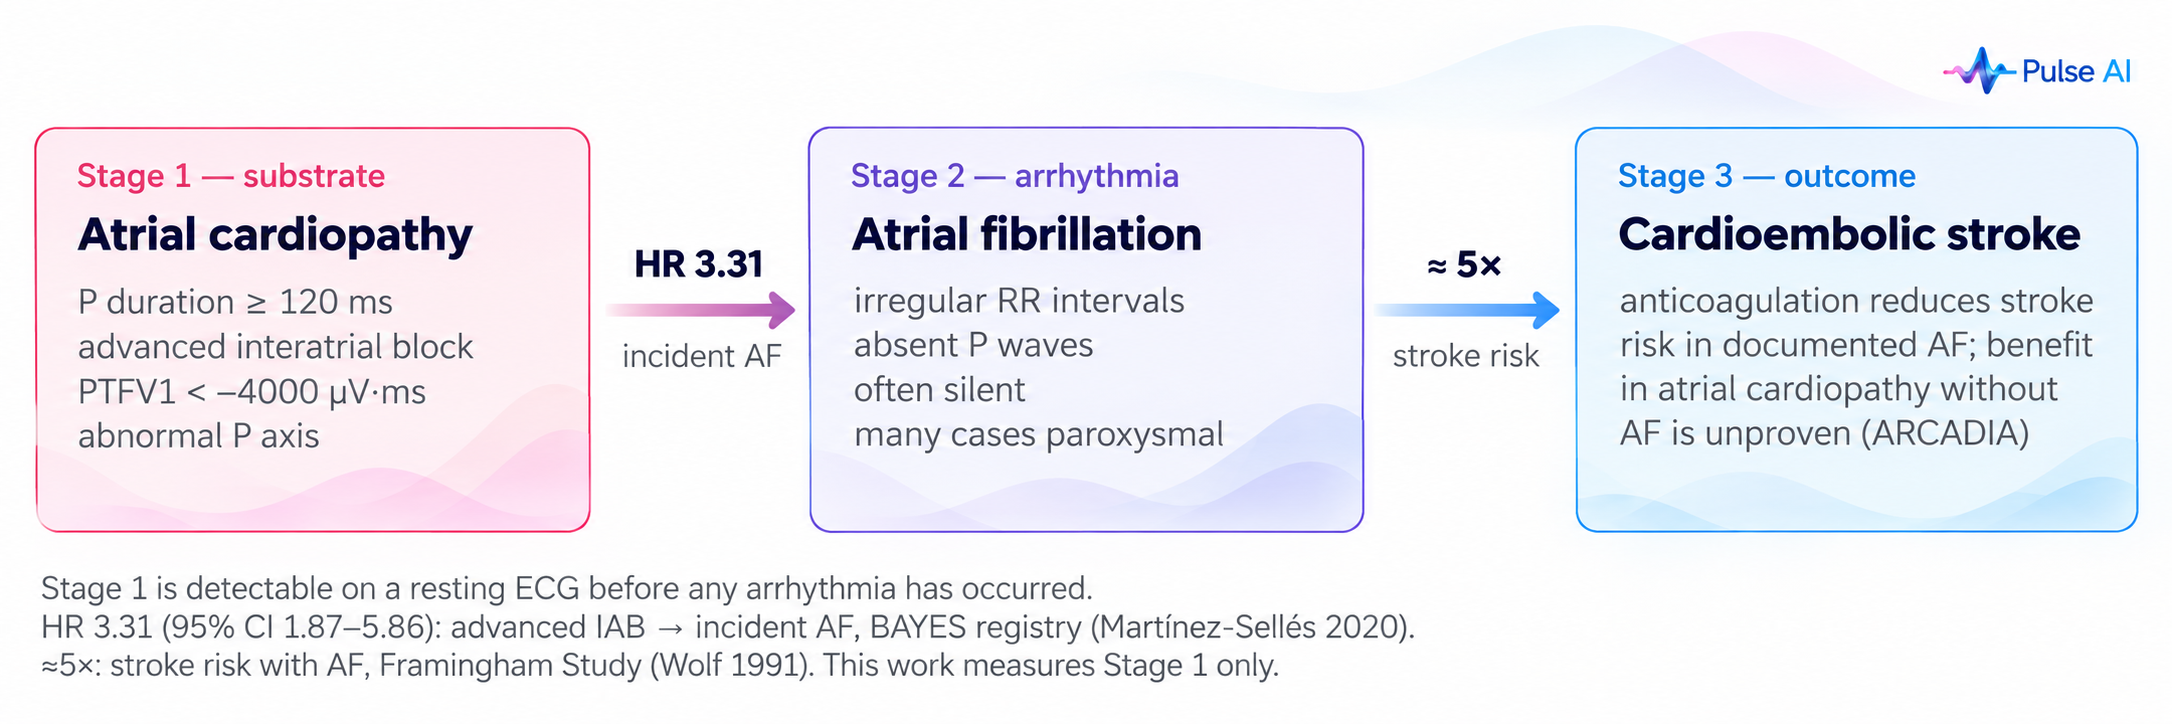
\includegraphics[width=\textwidth]{fig03_chain_v1.png}
\caption{The three-stage chain from atrial damage to stroke. PULSE-AI v1 measures
Stage~1 only and makes no treatment claim.}
\label{fig:chain}
\end{figure*}

% ===========================================================================
\section{Related Work}

\textit{Wave-boundary detection.} The wavelet method of Mart\'{\i}nez et
al.~\cite{martinez2004wavedet} and the multilead rule of Laguna et
al.~\cite{laguna1994multilead} are standard methods. Both were tested on the QT
Database (QTDB)~\cite{laguna1997qtdb} against the tolerances of the Common
Standards for Electrocardiography (CSE) project~\cite{cse1985standards}. The
Lobachevsky University Database (LUDB) gives expert boundaries for all 12
leads~\cite{kalyakulina2020ludb}.

\textit{P-wave reference values.} Normal values of P duration depend on how it is
measured. Measuring across all leads at once gives longer durations than reading
one lead~\cite{kligfield2007aha1}. With a lead-independent algorithm, the median P
duration of healthy men aged 60--89 is about 120\,ms~\cite{rijnbeek2014normal}.
P duration increases with age~\cite{havmoller2007pwave}, and in a large
primary-care cohort both short and long P waves were linked to
AF~\cite{nielsen2015pwave}. The MVP score combines P-wave shape, voltage and
duration into one number~\cite{alexander2019mvp}.

\textit{Learned ECG models.} PTB-XL~\cite{wagner2020ptbxl} is the standard public
data set for 12-lead ECG classification. Deep models reach high accuracy on it,
but they do not output quantities a doctor can check~\cite{attia2019af}.

% ===========================================================================
\section{Methods}

Table~\ref{tab:abbr} lists the abbreviations used in this paper.

\begin{table}[!t]
\caption{Abbreviations}
\label{tab:abbr}
\centering
\footnotesize
\setlength{\tabcolsep}{3pt}
\begin{tabular}{@{}ll@{\hspace{8pt}}ll@{}}
\toprule
AF & atrial fibrillation & LUDB & Lobachevsky Univ.\ Database \\
AUROC & area under ROC curve & MVP & morphology-voltage-P score \\
AUPRC & area under prec.--recall curve & OLS & ordinary least squares \\
BH & Benjamini--Hochberg & PPG & photoplethysmography \\
CI & confidence interval & PTFV1 & P-terminal force in V1 \\
CSE & Common Standards for ECG & QC & quality control \\
ECG & electrocardiogram & QTc & heart-rate-corrected QT \\
HR & heart rate & QTDB & QT Database \\
IAB & interatrial block & RMSSD & root mean square of \\
IQR & interquartile range & & successive RR differences \\
LAE & left atrial enlargement & SMD & standardised mean diff. \\
LAO & left atrial overload & Tpe & T-peak to T-end interval \\
\bottomrule
\end{tabular}
\end{table}

\begin{figure*}[!t]
\centering
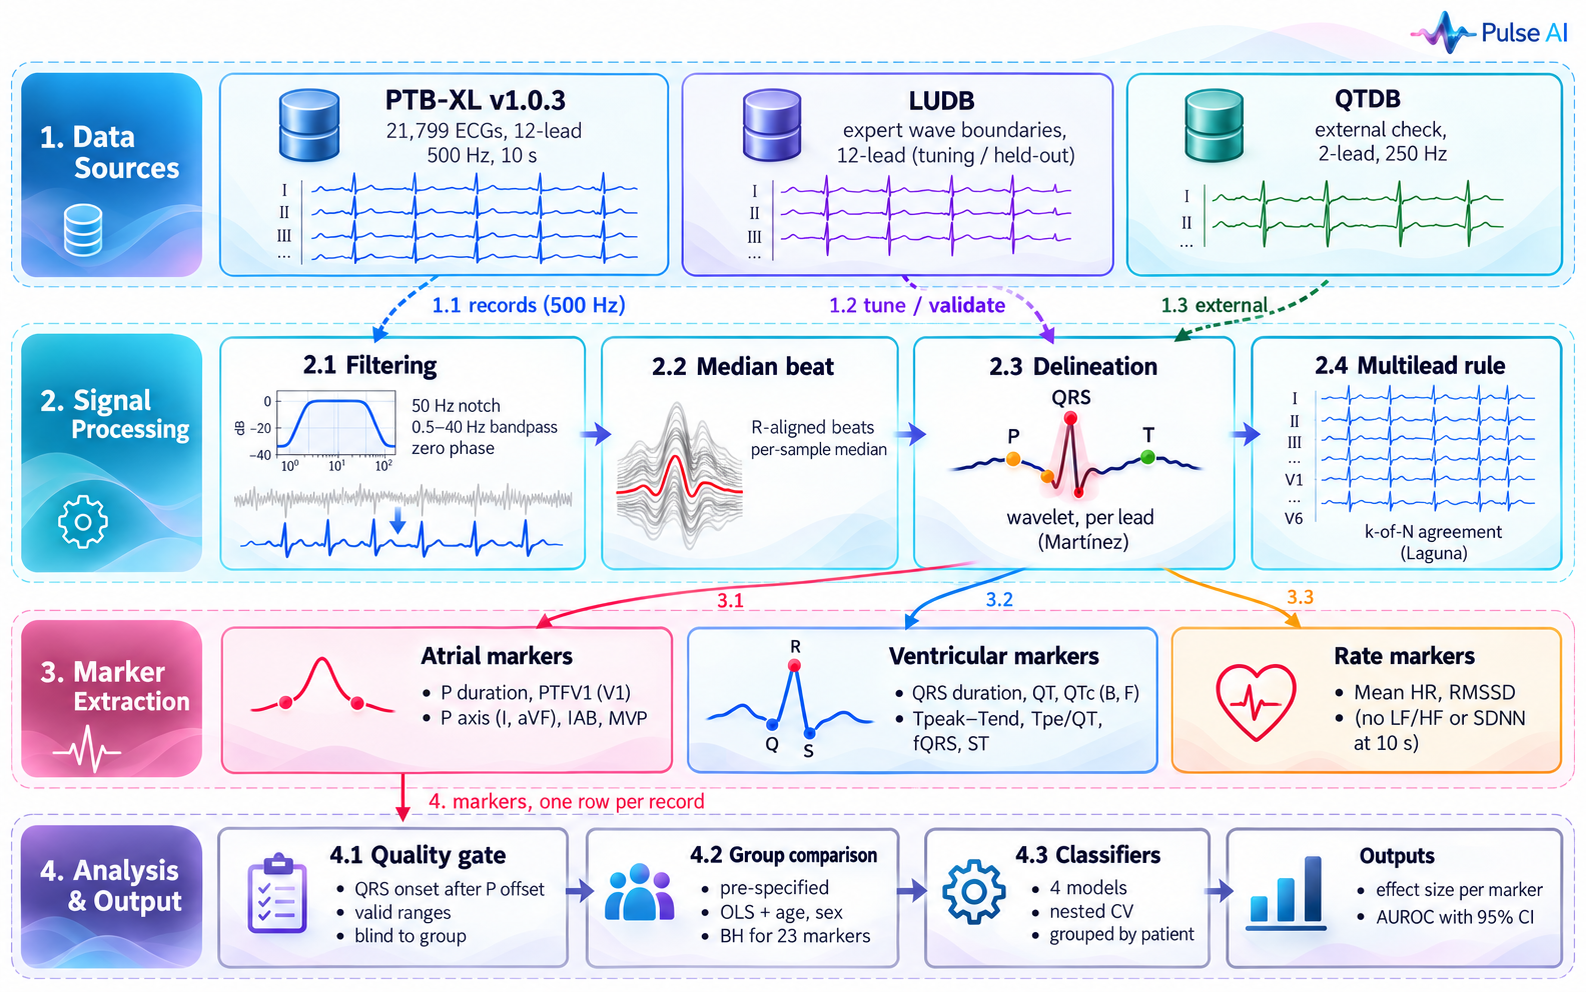
\includegraphics[width=0.86\textwidth]{fig02_pipeline_v1.png}
\caption{PULSE-AI v1 pipeline. Numbers on the arrows give the order of
operations. Dashed arrows: data used only to tune and test the boundary
detector. Red: atrial markers; blue: ventricular markers; orange: rate markers.
Waveforms and icons are schematic.}
\label{fig:pipeline}
\end{figure*}

\subsection{Data and Cohort}

PTB-XL v1.0.3~\cite{wagner2020ptbxl} contains 21{,}799 ECGs of 10\,s from 18{,}869
patients; we used the files sampled at 500\,Hz. Cases were sinus-rhythm ECGs
carrying the diagnostic label LAO/LAE (left atrial overload or enlargement).
Controls were sinus-rhythm ECGs of patients who never carry that label. We used
one ECG per patient and matched two controls to each case, exactly on sex and
within $\pm$5 years of age, keeping patients aged 40 or over. Of \nNEligCase{}
eligible cases, \nAgeLostCase{} were younger than 40; every remaining case was
matched, giving \nNMatchCase{} cases and \nNMatchCtrl{} controls with a mean age
of \nAgeMatched{} years. Left ventricular hypertrophy (LVH), bundle branch block,
Wolff--Parkinson--White pattern and paced rhythm were not exclusion criteria;
their effect was tested afterwards (Section~\ref{sec:sens}). A second design
(Design~B) used the sinus-rhythm ECGs of patients who had AF recorded in another
PTB-XL ECG (\nNBCaseMatched{} cases, \nNBCtrlMatched{} controls). The sinus ECG
could lie before or after the AF ECG (\nBBefore{} and \nBAfter{} of the
\nNBCaseMatched{} cases), so Design~B tests association with an AF history, not
prediction of future AF. All data splits were grouped by patient, so no patient appears in both
training and test data.

\subsection{Filtering and Median Beat}

Each lead $x_\ell[n]$, $\ell=1,\dots,12$, was filtered with a 50\,Hz notch
($Q=30$) and a 0.5--40\,Hz fourth-order Butterworth band-pass $h[n]$. PTB-XL was
recorded on 50\,Hz mains; the band-pass alone already attenuates 50\,Hz by
\nNotchBpDb\,dB, and the raw records showed a median 50\,Hz peak only
\nNotchMedDb\,dB above the neighbouring noise floor, so the notch is a safeguard
for the few noisy records (\nNotchOverTen{} with a peak above 10\,dB). The filter was applied
forward and backward,
\begin{equation}
y_\ell[n] = h[-n] * \big(h[n] * x_\ell[n]\big), \qquad
Y_\ell(e^{j\omega}) = |H(e^{j\omega})|^2\, X_\ell(e^{j\omega}),
\end{equation}
which gives zero phase shift, so wave boundaries are not moved in time. R peaks
$r_1,\dots,r_K$ were found on all leads together, and a median beat was formed
for each lead,
\begin{equation}
\bar{y}_\ell[n] = \median_{k=1,\dots,K}\; y_\ell[r_k+n], \qquad
-0.40f_s \le n \le 0.50f_s ,
\end{equation}
with $f_s=500$\,Hz. Noise varies from beat to beat and is suppressed by the
median, while the P wave, which appears at the same position in every sinus
beat, is kept. Premature or ectopic beats were not removed before averaging; the
median tolerates them only while they are a minority of the beats, and mean HR,
RMSSD and the RR used for QTc include every interval.

\subsection{Wave-Boundary Detection and Its Validation}

Each median beat was analysed with the dyadic wavelet transform of
Mart\'{\i}nez et al.~\cite{martinez2004wavedet},
\begin{equation}
W_{2^k}\bar{y}[n] = \sum_m \bar{y}[m]\,\psi_{2^k}[n-m], \qquad k=1,\dots,5,
\end{equation}
where $\psi$ is the derivative of a quadratic spline, so each scale behaves as a
smoothed derivative. A wave is accepted when $|W_{2^k}\bar{y}|$ exceeds a
threshold proportional to its root-mean-square value; its peak lies at a zero
crossing of $W_{2^k}\bar{y}$ and its onset and offset where the modulus falls
below a fixed fraction of the neighbouring maximum. The boundaries found in the
12 leads were combined with the $k$-of-$N$ rule of Laguna et
al.~\cite{laguna1994multilead}: a global onset is the earliest time at which at
least $k$ leads agree within $\delta$\,ms ($k=3$ for QRS and T; $k=2$,
$\delta=10$\,ms for P). Our changes to the published method (search windows, a
0.02\,mV minimum P-wave height and a 100\,ms P-wave slope span) are documented
in the code. LUDB~\cite{kalyakulina2020ludb} was split by record into a tuning
half and a held-out half. Every parameter was set on the tuning half only, and
all accuracy figures are from held-out sinus-rhythm records. QTDB served as an
external check with no tuning: it was processed at its native 250\,Hz, the rate
at which the wavelet scales are defined~\cite{martinez2004wavedet}, using both
leads and the first cardiologist's annotation (q1c); \nQtdbScored{} of
\nQtdbListed{} records (\nQtdbBeats{} beats) were scored, one having no annotated
QRS. Synthetic ECGs built from half-sine waves with exactly known boundaries were
used only for unit tests and to measure systematic bias of the detector, never
in any group analysis.

\subsection{Markers}

Table~\ref{tab:markers} lists the markers. With $t_\text{on}$ and $t_\text{off}$
the global boundaries, the main markers are
\begin{align}
\text{P duration} &= t^{P}_\text{off}-t^{P}_\text{on}, \\
\text{PTFV1} &= -A_\text{neg}\times D_\text{neg} \quad [\mu\text{V}\cdot\text{ms}], \\
\theta_P &= \operatorname{atan2}\!\big(\tfrac{2}{\sqrt{3}}\,S_\text{aVF},\; S_\text{I}\big), \\
\text{QTc}_\text{B} = \frac{\text{QT}}{\sqrt{\text{RR}}}, &\qquad
\text{QTc}_\text{F} = \frac{\text{QT}}{\sqrt[3]{\text{RR}}}, \\
\text{RMSSD} &= \sqrt{\tfrac{1}{N-1}\textstyle\sum_{i=1}^{N-1}(\text{RR}_{i+1}-\text{RR}_i)^2},
\end{align}
where $A_\text{neg}$ and $D_\text{neg}$ are the depth and duration of the
terminal negative part of the P wave in V1 (measured with V1's own boundaries),
$S_\text{I}$ and $S_\text{aVF}$ are the P-wave areas in leads I and aVF (the
factor $2/\sqrt{3}$ follows from the hexaxial lead geometry), and RR is the mean
beat interval in seconds. Fragmented QRS (fQRS) is read from a separate
0.5--100\,Hz median beat, because the 40\,Hz low-pass would smooth the notches it
looks for. Tpe runs from the maximum of the spatial magnitude
$\sqrt{\sum_\ell \bar{y}_\ell^2[n]}$ in the T wave to the T offset. IAB is
reported only descriptively. QTc is analysed as a continuous value; the single
460\,ms threshold in Table~\ref{tab:markers} is the female limit of
\cite{rautaharju2009aha4} applied to both sexes and is not used in any test.
Heart-rate-variability measures that need at least
300\,s of signal (SDNN, LF/HF, sample entropy, DFA)~\cite{taskforce1996hrv} are
not computed on 10-s records. If a record lacks a required lead, the marker is
returned as ``not applicable'' with the reason, so a single-lead recording skips
PTFV1 automatically.

\begin{table}[!t]
\caption{Markers, leads used and published thresholds}
\label{tab:markers}
\centering
\footnotesize
\setlength{\tabcolsep}{3pt}
\begin{tabular}{@{}llll@{}}
\toprule
Marker & Leads & Abnormal & Ref. \\
\midrule
\multicolumn{4}{@{}l}{\textit{Atrial}}\\
P duration & all 12 & $\geq$120\,ms & \cite{bayesdeluna2012iab} \\
PTFV1 & V1 & $\leq-4000$\uVms & \cite{morris1964ptfv1} \\
P axis & I, aVF & outside 0--75$^\circ$ & \cite{maheshwari2017paxis} \\
IAB class & II, III, aVF & P $\geq$120\,ms ($\pm$ biphasic) & \cite{bayesdeluna2012iab} \\
MVP score & 12 & $\geq$5 of 6 & \cite{alexander2019mvp} \\
\multicolumn{4}{@{}l}{\textit{Ventricular}}\\
QRS duration & all 12 & $\geq$120\,ms & \cite{surawicz2009aha3} \\
QTc (B, F) & all 12 & $\geq$460\,ms & \cite{rautaharju2009aha4,bazett1920qt,fridericia1920qt} \\
Tpe, Tpe/QT & all 12 & Tpe/QT $>$0.25 & \cite{gupta2008tpe} \\
fQRS & territories & $\geq$2 leads & \cite{das2006fqrs} \\
ST at J$+$60\,ms & each lead & --- & --- \\
\multicolumn{4}{@{}l}{\textit{Rate}}\\
Mean HR, RMSSD & 12 & --- & \cite{taskforce1996hrv} \\
\bottomrule
\end{tabular}
\end{table}

\subsection{Quality Control}

A record was excluded if a required marker was missing, if HR, QRS, QT or P
duration was outside physiological limits, or if the detected QRS onset came
before the P offset on the median beat. The last case cannot occur in a real
heart and shows that the boundaries were placed wrongly. The quality check
receives only the measurements of a record, never its group label (this is
enforced by a unit test), and every exclusion is counted under a named rule.

\subsection{Statistical Analysis Fixed in Advance}

The analysis plan was written and saved before any group difference was
computed. The primary endpoint was P duration, treated as a continuous value and
modelled by ordinary least squares,
\begin{equation}
m_i = \beta_0 + \beta_1\,\text{case}_i + \beta_2\,\text{age}_i + \beta_3\,\text{sex}_i + \varepsilon_i ,
\end{equation}
where $\beta_1$ is the adjusted difference between cases and controls. Matched
sets broken by the quality check were analysed unmatched, with age and sex in
the model. Effect sizes were Hedges' $g$,
\begin{equation}
g = \Big(1-\frac{3}{4(n_1+n_2)-9}\Big)\frac{\bar{m}_1-\bar{m}_2}{s_p},
\end{equation}
with $s_p$ the pooled standard deviation, and Cliff's $\delta$. The \nNSec{}
secondary markers used the same model, with the false discovery rate held at 5\%
by the Benjamini--Hochberg (BH) procedure. Threshold calls (IAB, abnormal PTFV1,
high MVP) were reported as percentages only. LAE labels in PTB-XL are given
partly from P-wave criteria, so a difference in P-wave markers confirms that our
measurement agrees with the label rather than discovering something new.
Markers outside the LAE definition do not have this problem. Sensitivity
analyses used the complete matched sets (paired test) and Design~B. Checks
added after the plan, and labelled post hoc wherever they appear, were: reports
confirmed by a cardiologist only; exclusion of, or adjustment for, LVH and
conduction disease; a comparison of included and excluded records; and a
validation of PTFV1 against expert V1 boundaries.

\subsection{Classifiers (Exploratory)}

This part was added after the plan and is reported as exploratory. Four models
were compared: L2-regularised logistic regression, a decision tree of depth 2--5,
a random forest and histogram gradient boosting. Nested cross-validation was
used: an outer 5-fold split, stratified and grouped by patient, measured
performance, and an inner 3-fold split chose the hyperparameters and the
decision threshold (Youden's $J$). Missing-value filling and scaling were fitted
inside each training fold only. Feature set~A held all markers plus age and sex.
Set~B removed every marker derived from the P wave (P duration, PTFV1, P axis,
IAB, MVP), so its result cannot come from the information used to assign the
label. Discrimination was measured by
\begin{equation}
\text{AUROC} = P\big(\hat{s}_\text{case} > \hat{s}_\text{control}\big),
\end{equation}
the probability that a random case scores above a random control, and by the
AUPRC, both with 1000-sample bootstrap CIs and beside a model that always
predicts ``control''. The whole nested procedure was repeated on \nNPerm{}
random shuffles of the labels, giving $p=(1+\#\{\text{AUROC}_\text{perm}\ge
\text{AUROC}\})/(1+\nNPerm)$. Deep neural networks were not used on purpose:
with $n=\nNAll$ they cannot be trained reliably and would not give readable
outputs.

\subsection{Software}
\label{sec:software}

Each marker is declared once in code together with its leads, units, normal
range, threshold and reference. The quality check, Table~\ref{tab:markers} and
the device-capability map are generated from these declarations, and every
number in this paper is produced by a script from saved results. The code,
analysis plan and result files are available at
\url{https://github.com/Huzaimkk/pulse-ai-v1}.

% ===========================================================================
\section{Results}

\subsection{Cohort}

Of \nNMatchAll{} matched ECGs, \nNExcl{} (\nPctExcl\%) were excluded
(Fig.~\ref{fig:flow}). The main reason was a QRS onset placed before the P offset
(\nNOverlap{} ECGs; \nPctOverlapCase\% of cases and \nPctOverlapCtrl\% of
controls). \nNCase{} cases and \nNCtrl{} controls remained, and they were still
balanced in age (\nAgeCase{}~$\pm$~\nAgeCaseSd{} vs.\
\nAgeCtrl{}~$\pm$~\nAgeCtrlSd{} years, standardised mean difference \nSmdAge) and
sex (\nMaleCase\% vs.\ \nMaleCtrl\% male, \nSmdMale). The exclusion rate was the
same in both groups (\nQcRateCase\% vs.\ \nQcRateCtrl\%, $p=\nQcRateP$; post hoc),
and excluded ECGs did not differ from included ones in age, sex, HR or number of
beats. They did have longer P, QRS and QTc values, as expected, since these are
the values the quality rules test.

\begin{figure}[!t]
\centering
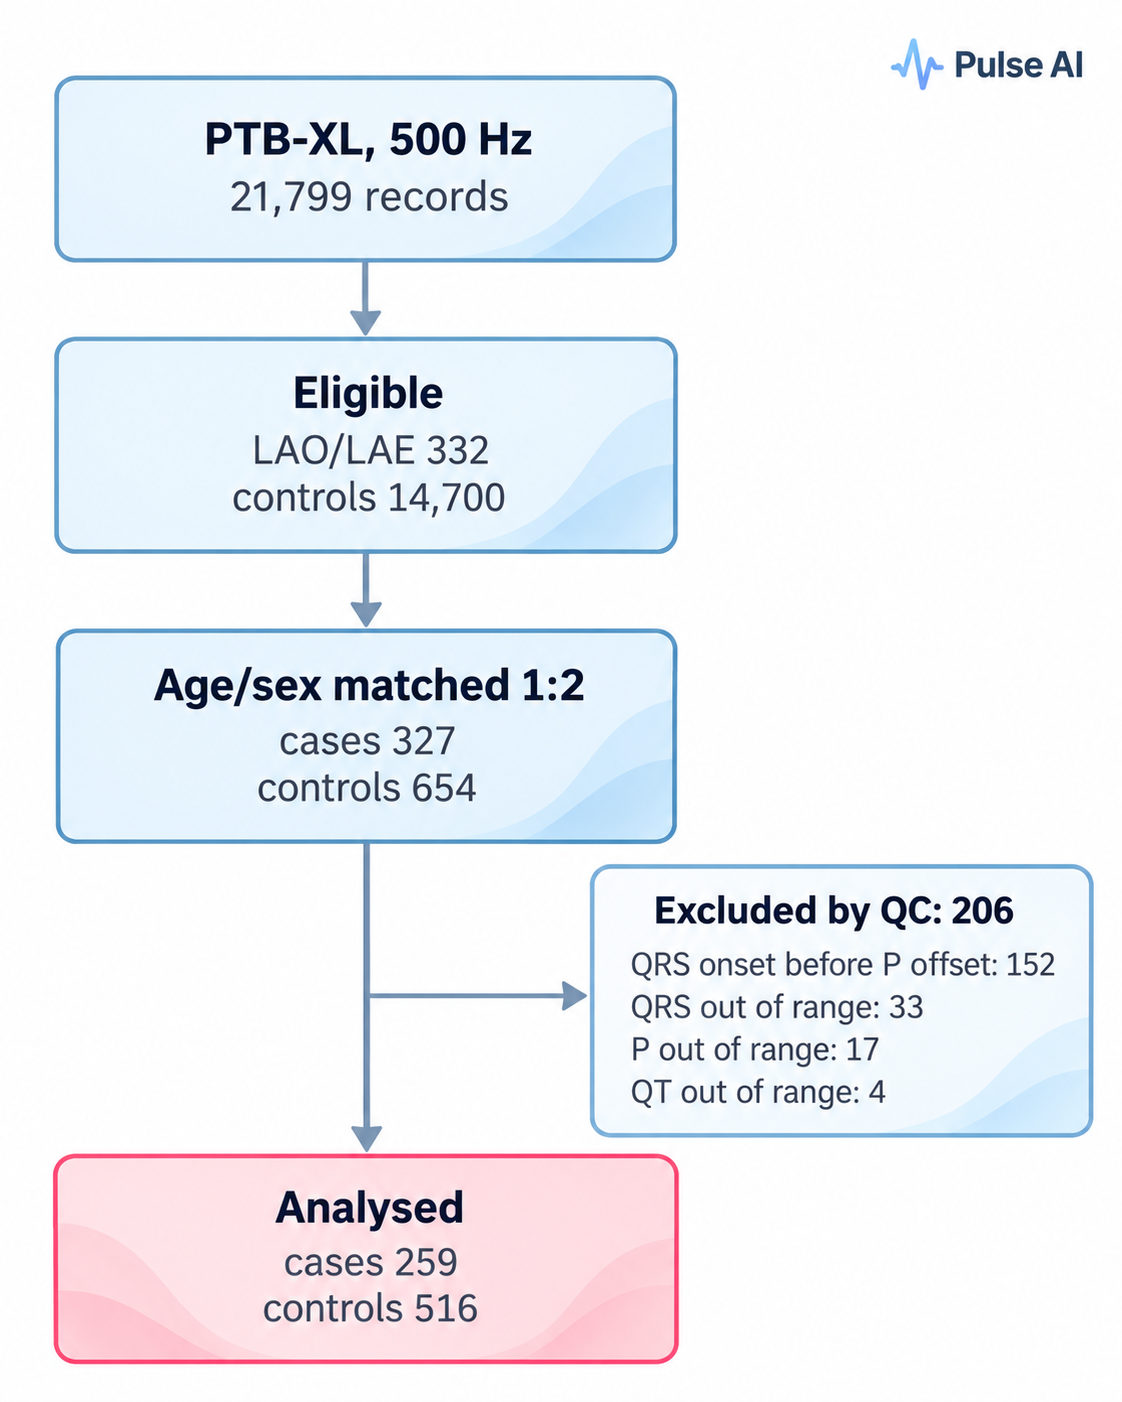
\includegraphics[width=0.62\columnwidth]{fig04_flow_v1.png}
\caption{Cohort flow. Each excluded ECG is counted under the first rule it
failed.}
\label{fig:flow}
\end{figure}

\subsection{Accuracy of Wave-Boundary Detection}

On \nNLudbRec{} held-out LUDB sinus records (\nNLudbBeats{} scored P waves, P-wave
detection \nPSens\%), the within-record standard deviations of the boundary error
were \nSdPon, \nSdPoff, \nSdQon, \nSdQoff{} and \nSdToff\,ms for P onset,
P offset, QRS onset, QRS offset and T offset (Table~\ref{tab:delin}). P offset,
QRS offset and T offset met the CSE tolerances; P onset and QRS onset did not.
For each record, the error in P duration was \nGTwoBias{}~$\pm$~\nGTwoBiasSd\,ms
(mean absolute error \nGTwoMae\,ms), and \nQtdbBias{}~$\pm$~\nQtdbBiasSd\,ms on
QTDB. Beat by beat, 95\% of the errors lay between \nBaLo{} and \nBaHi\,ms
(Fig.~\ref{fig:ba}, limits of agreement = bias $\pm 1.96$\,SD). Agreement on the
120\,ms yes/no decision was low (Cohen's $\kappa=\nGTwoKappa$), partly because the
expert reference itself placed \nGTwoRefPrev\% of LUDB sinus records at or above
120\,ms. On synthetic ECGs the measured P duration followed
$\nCompSlope\times\text{true}+\nCompIcpt$\,ms, so true differences between
groups are slightly reduced in our measurements.

PTFV1 uses V1's own boundaries, which were checked separately (post hoc) against
the expert V1 marks on the same \nVOffN{} held-out records. V1 P onset agreed
(\nVOnBias~$\pm$~\nVOnSd\,ms), but our V1 P offset was late by
\nVOffBias~$\pm$~\nVOffSd\,ms. This lengthens the terminal negative part
(\nVTermDur\,ms) without changing its depth (\nVTermDepth\,\textmu V). PTFV1
computed with our boundaries and with the expert boundaries on the same signal
agreed well as a continuous value (ICC \nVIcc, Spearman $\rho=\nVRho$; bias
\nVPtfBias\uVms), and the abnormal call agreed with $\kappa=\nVKappa$. All
disagreements went one way: \nVOursOnly{} records called abnormal by us were
normal with expert boundaries, and \nVLudbOnly{} the other way (\nVAbnOurs\% vs.\
\nVAbnLudb\% abnormal). PTFV1 is therefore reliable as a continuous measure, but
its threshold call over-reports.

\begin{table}[!t]
\caption{Boundary error on held-out LUDB sinus records (ms)}
\label{tab:delin}
\centering
\footnotesize
\begin{tabular}{@{}lrrrr@{}}
\toprule
Boundary & Mean & SD$_{\text{within}}$ & CSE limit & Ref.~\cite{martinez2004wavedet} \\
\midrule
P onset & \nMeanPon & \nSdPon & \nCsePon & \nMartPon \\
P offset & \nMeanPoff & \nSdPoff & \nCsePoff & \nMartPoff \\
QRS onset & \nMeanQon & \nSdQon & \nCseQon & \nMartQon \\
QRS offset & \nMeanQoff & \nSdQoff & \nCseQoff & \nMartQoff \\
T offset & \nMeanToff & \nSdToff & \nCseToff & \nMartToff \\
\bottomrule
\end{tabular}

\vspace{2pt}
\parbox{\columnwidth}{\scriptsize SD$_{\text{within}}$: mean of the per-record
standard deviations, the statistic used in~\cite{martinez2004wavedet}. Their
values (QTDB, best lead per point) are shown for orientation only.}
\end{table}

\begin{figure}[!t]
\centering
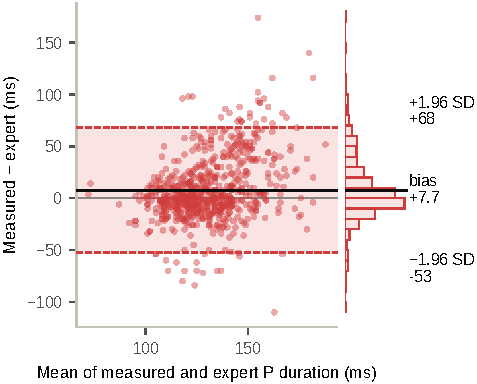
\includegraphics[width=0.85\columnwidth]{fig05_bland_altman}
\caption{Bland--Altman plot of measured P duration against expert annotation,
held-out LUDB sinus beats. Shaded band: 95\% limits of agreement
(\nBaLo{} to \nBaHi\,ms).}
\label{fig:ba}
\end{figure}

\subsection{Calibration on PTB-XL}

Compared with normal ranges taken from single-lead reading (P 80--120\,ms, QRS
70--110\,ms), the cohort medians of P duration (\nMedP\,ms) and QRS duration
(\nMedQ\,ms) looked abnormal. Compared with normal values measured the same way
and in the same age range~\cite{rijnbeek2014normal}, the remaining offsets were
\nOffPLo--\nOffPHi\,ms for P and \nOffQLo--\nOffQHi\,ms for QRS, and similar in men
and women. A constant offset moves cases and controls by the same amount. It
makes absolute values and fixed thresholds unreliable, but it does not affect the
comparison between groups. PR, QT and HR were within published ranges.

\subsection{Case--Control Comparison}

The primary endpoint showed no difference (Fig.~\ref{fig:dist}). Median P
duration was \nPdCaseMed{} ms in cases and \nPdCtrlMed{} ms in controls; the
adjusted difference was \nPrimDiff\,ms (95\% CI \nPrimLo{} to \nPrimHi;
$p=\nPrimP$; $g=\nPrimG$). The 120\,ms threshold marked \nIabCase\% of cases and
\nIabCtrl\% of controls as IAB, and the high-risk MVP group held \nMvpHiCase\% and
\nMvpHiCtrl\%.

PTFV1 behaved differently. It was more negative in cases by \nDiffPtf\uVms{} (95\%
CI \nLoPtf{} to \nHiPtf; $g=\nGPtf$; $q\nQPtf$), and \nPtfAbCase\% of cases
against \nPtfAbCtrl\% of controls passed the abnormal threshold. These
percentages are descriptive only: they include the over-calling shown above, and
PTB-XL controls also had deeper terminal negative P waves than LUDB records
(median \nCtlTermDepth{} vs.\ \nLudbTermDepth\,\textmu V), which boundary error
cannot cause. Of the \nNSec{}
secondary markers, \nNSecSig{} differed at $q<0.05$ (Fig.~\ref{fig:forest}).
Among markers outside the LAE definition, cases had a longer QRS
(\nDiffQrs\,ms, $g=\nGQrs$), longer QTc (Fridericia, \nDiffQtcF\,ms, $g=\nGQtcF$),
longer Tpe (\nDiffTpe\,ms), higher HR (\nDiffHr\,bpm), ST depression in I, aVL, V5
and V6 ($g=\nGStVsix$ in V6) and ST elevation in aVR and V1--V3.

\begin{figure*}[!t]
\centering
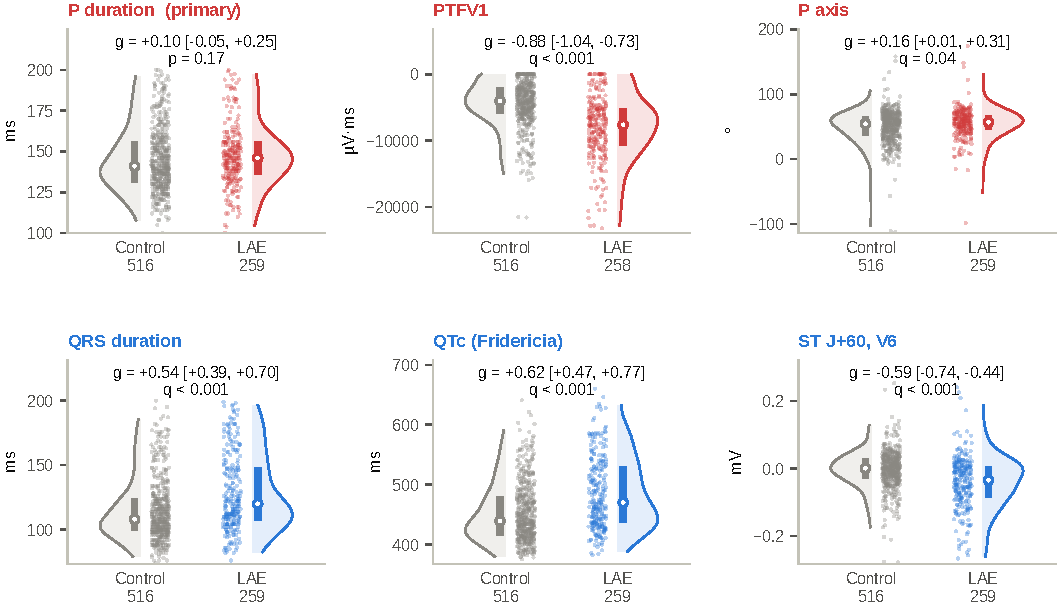
\includegraphics[width=0.80\textwidth]{fig06_distributions}
\caption{Distribution of three atrial markers (top) and three ventricular
markers (bottom) in cases (coloured) and controls (grey). Each dot is one ECG;
the half-violin shows the density, the bar the IQR and the circle the median.
Hedges' $g$ with 95\% CI; $p$ for the primary endpoint and BH-adjusted $q$ for
secondary markers.}
\label{fig:dist}
\end{figure*}

\begin{figure}[!t]
\centering
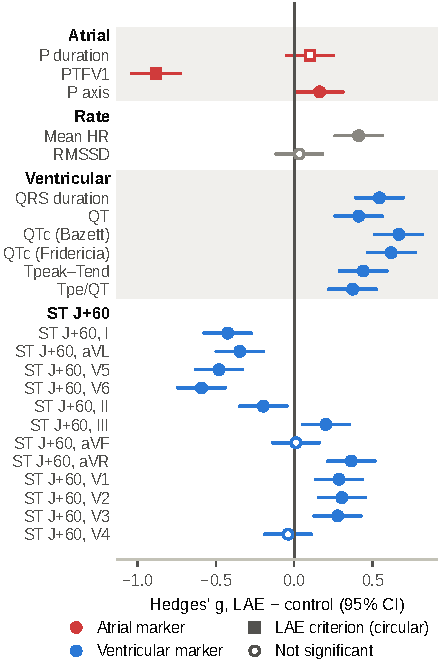
\includegraphics[width=0.72\columnwidth]{fig07_effect_sizes}
\caption{Adjusted effect size of every marker. Squares: markers that are part
of the LAE definition. Open symbols: not significant. The number of beats,
a quality covariate counted among the \nNSec{} secondary markers, is not
plotted.}
\label{fig:forest}
\end{figure}

\subsection{Sensitivity Analyses}
\label{sec:sens}

In the \nSOneN{} complete matched sets the paired difference in P duration was
\nSOneDiff\,ms (\nSOneLo{} to \nSOneHi; $p=\nSOneP$). Using only reports confirmed
by a cardiologist (\nNHumanCase{} cases, \nNHumanCtrl{} controls) it was \nHvDiff\,ms
(\nHvLo{} to \nHvHi; $p=\nHvP$). In Design~B, where the case label (AF in another
ECG) does not depend on the P wave, P duration was longer in cases by
\nBDiff\,ms (\nBLo{} to \nBHi; $p=\nBP$; $g=\nBG$; \nBCase{} cases, \nBCtrl{}
controls); as noted above, this is an association with AF history.

LVH was more common in cases than controls (\nPrevLvhCase\% vs.\
\nPrevLvhCtrl\%), as were left (\nPrevLbbbCase\% vs.\ \nPrevLbbbCtrl\%) and right
(\nPrevRbbbCase\% vs.\ \nPrevRbbbCtrl\%) bundle branch block. Two post-hoc checks
(Table~\ref{tab:lvh}) refitted the model (a) after removing every ECG with LVH,
complete bundle branch block, WPW or pacing (\nExDropCase{} cases and
\nExDropCtrl{} controls) and (b) with LVH as an extra covariate. PTFV1, QRS,
QTc and HR kept their direction and significance in both. The QRS difference
fell from \nDiffQrs{} to \nExQrsDiff\,ms in (a), so part of it came from these
conditions. P duration stayed non-significant with LVH as a covariate; in the
unmatched subset (a) it reached \nExPDiff\,ms ($p=\nExPP$, uncorrected), which we
do not treat as a finding.

\begin{table}[!t]
\caption{Post-hoc check for LVH and conduction disease: adjusted case--control
difference (95\% CI)}
\label{tab:lvh}
\centering
\scriptsize
\setlength{\tabcolsep}{2pt}
\resizebox{\columnwidth}{!}{%
\begin{tabular}{@{}lccc@{}}
\toprule
Marker & Original & (a) excluded & (b) LVH covariate \\
 & \nNCase/\nNCtrl & \nExN/\nExNCtrl & \nNCase/\nNCtrl \\
\midrule
P dur.\ (ms) & \nPrimDiff{} (\nPrimLo, \nPrimHi) & \nExPDiff{} (\nExPLo, \nExPHi) & \nCovPDiff{} (\nCovPLo, \nCovPHi) \\
PTFV1 (\uVms) & \nDiffPtf{} (\nLoPtf, \nHiPtf) & \nExPtfDiff{} (\nExPtfLo, \nExPtfHi) & \nCovPtfDiff{} (\nCovPtfLo, \nCovPtfHi) \\
QRS (ms) & \nDiffQrs{} (\nLoQrs, \nHiQrs) & \nExQrsDiff{} (\nExQrsLo, \nExQrsHi) & \nCovQrsDiff{} (\nCovQrsLo, \nCovQrsHi) \\
QTcF (ms) & \nDiffQtcF{} (\nLoQtcF, \nHiQtcF) & \nExQtcFDiff{} (\nExQtcFLo, \nExQtcFHi) & \nCovQtcFDiff{} (\nCovQtcFLo, \nCovQtcFHi) \\
HR (bpm) & \nDiffHr{} (\nLoHr, \nHiHr) & \nExHrDiff{} (\nExHrLo, \nExHrHi) & \nCovHrDiff{} (\nCovHrLo, \nCovHrHi) \\
\bottomrule
\end{tabular}}

\vspace{2pt}
\parbox{\columnwidth}{\scriptsize (a) ECGs with LVH, complete bundle branch block,
WPW or pacing removed from both groups, not re-matched. Model: marker $\sim$ group
+ age + sex (+ LVH in b).}
\end{table}

\subsection{Classifiers}

Table~\ref{tab:models} and Fig.~\ref{fig:roc} give the results. With all markers
(set~A), the random forest reached an AUROC of \nAucRfA{} (\nAucLoRfA--\nAucHiRfA);
logistic regression was close behind (\nAucLrA). Without any P-wave marker
(set~B), the best AUROC was \nAucRfB{} (\nAucLoRfB--\nAucHiRfB). None of the
\nNPerm{} label shuffles reached the observed AUROC in either set (highest
\nNullMax; $p=\nPermP$, the smallest value possible with \nNPerm{} shuffles). At
the threshold chosen in the inner loop, the set-A forest had a sensitivity of
\nSensRfA{} and a specificity of \nSpecRfA{} (true positives \nTp, false negatives
\nFn, false positives \nFp, true negatives \nTn). Its accuracy of \nAccRfA{}
should be read against \nAccMajA{} for a model that always answers ``control'';
this is why accuracy is not the main measure. PTFV1 was the most important
marker in set~A; in set~B the leading markers were ST in V6, QRS duration and QTc
(Fig.~\ref{fig:imp}). Because QT, QTcB, QTcF and Tpe/QT are strongly
correlated, shuffling them one at a time understates them. Shuffled together
(post hoc), the QT family lowered AUROC by \nGiQtA{} in set~A and \nGiQtB{} in
set~B, against \nGiQtSumA{} and \nGiQtSumB{} for the sum of its single-marker
values; the P-wave family lowered it by \nGiPA{} in set~A, almost all from
PTFV1.

\begin{table}[!t]
\caption{Classifier results, nested cross-validation, LAE vs.\ control
($n=\nNAll$, prevalence \nPrev)}
\label{tab:models}
\centering
\footnotesize
\setlength{\tabcolsep}{2.5pt}
\begin{tabular}{@{}llcccc@{}}
\toprule
Set & Model & AUROC (95\% CI) & AUPRC & Sens & Spec \\
\midrule
\multirow{4}{*}{A} & Logistic & \nAucLrA{} (\nAucLoLrA--\nAucHiLrA) & \nPrcLrA & \nSensLrA & \nSpecLrA \\
 & Tree & \nAucDtA{} (\nAucLoDtA--\nAucHiDtA) & \nPrcDtA & \nSensDtA & \nSpecDtA \\
 & Forest & \textbf{\nAucRfA}{} (\nAucLoRfA--\nAucHiRfA) & \nPrcRfA & \nSensRfA & \nSpecRfA \\
 & Boosting & \nAucGbA{} (\nAucLoGbA--\nAucHiGbA) & \nPrcGbA & \nSensGbA & \nSpecGbA \\
\midrule
\multirow{4}{*}{B} & Logistic & \nAucLrB{} (\nAucLoLrB--\nAucHiLrB) & \nPrcLrB & \nSensLrB & \nSpecLrB \\
 & Tree & \nAucDtB{} (\nAucLoDtB--\nAucHiDtB) & \nPrcDtB & \nSensDtB & \nSpecDtB \\
 & Forest & \textbf{\nAucRfB}{} (\nAucLoRfB--\nAucHiRfB) & \nPrcRfB & \nSensRfB & \nSpecRfB \\
 & Boosting & \nAucGbB{} (\nAucLoGbB--\nAucHiGbB) & \nPrcGbB & \nSensGbB & \nSpecGbB \\
\midrule
 & Always ``control'' & 0.500 & \nPrev & 0.000 & 1.000 \\
\bottomrule
\end{tabular}

\vspace{2pt}
\parbox{\columnwidth}{\scriptsize Set A: all markers plus age and sex. Set B: set A
without any P-wave marker. Sensitivity and specificity at the threshold chosen in
the inner loop.}
\end{table}

\begin{figure*}[!t]
\centering
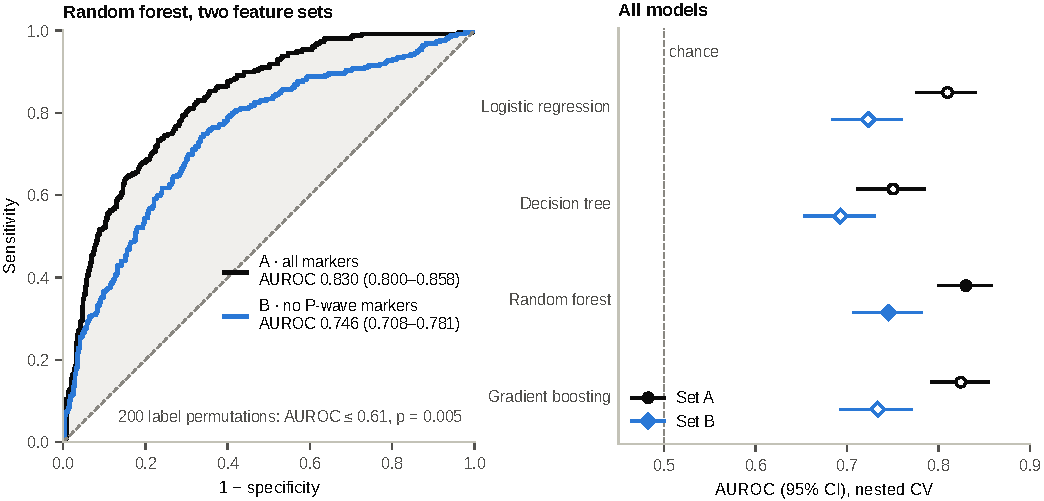
\includegraphics[width=0.66\textwidth]{fig08_roc}
\caption{Left: ROC curves of the random forest with and without P-wave markers
(pooled outer folds). Right: AUROC with 95\% CI for all four models.}
\label{fig:roc}
\end{figure*}

\begin{figure*}[!t]
\centering
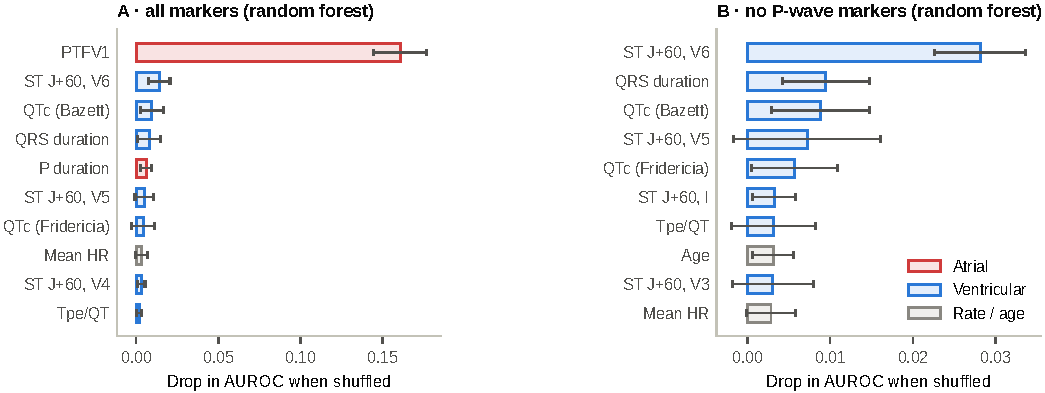
\includegraphics[width=0.62\textwidth]{fig09_importance}
\caption{Permutation importance (drop in outer-fold AUROC when a marker is
shuffled), random forest. Error bars: standard deviation over outer folds.}
\label{fig:imp}
\end{figure*}

% ===========================================================================
\section{Discussion}
\label{sec:disc}

\textit{Main findings.} PULSE-AI v1 measures named ECG markers automatically and
reports how accurate the measurement is. In an older hospital cohort these
markers separate expert-labelled LAE from matched controls, but not through P
duration, the marker usually mentioned first. P duration did not differ, and
the 120\,ms IAB threshold labelled more than nine in ten ECGs as abnormal in
\emph{both} groups. PTFV1 separated the groups.

\textit{Why P duration did not separate the groups.} We see three reasons. First,
normal values depend on how P duration is measured: measuring across all leads
gives longer values~\cite{kligfield2007aha1}, and with such methods healthy men
over 60 already have a median near 120\,ms~\cite{rijnbeek2014normal}. A 120\,ms
limit taken from visual reading~\cite{bayesdeluna2012iab} therefore cannot
separate groups whose mean age is 68. Second, our measurement has a positive
offset (\nOffPLo--\nOffPHi\,ms), a slope below one (\nCompSlope) and a per-record
error (SD \nGTwoBiasSd\,ms) that is large compared with the expected group
difference; all three push the result towards no difference. Third, the ECG
criteria for LAE include the negative end of the P wave in
V1~\cite{hancock2009aha5}, which is exactly what PTFV1 measures. In Design~B,
where the label does not come from the P wave, P duration was longer in cases
(\nBDiff\,ms). This suggests that P duration does follow atrial disease, but it
should be used as a calibrated continuous value and not as a yes/no call at
120\,ms.

\textit{The ventricular pattern.} A wider QRS, longer QTc, ST depression in the
lateral leads and ST elevation in aVR together form the ECG pattern of left
ventricular hypertrophy with strain, which often comes with high blood pressure
and an overloaded left atrium. These markers are not part of the LAE definition,
yet on their own they gave an AUROC of \nAucRfB. LVH was indeed three times as
common in cases, and removing it reduced the QRS difference but did not remove
it. The classifier is therefore not simply copying the label; the LAE label in
PTB-XL marks a wider heart condition.

\textit{Treatment.} The ARCADIA trial gave apixaban or aspirin to patients with
cryptogenic stroke and atrial cardiopathy, defined partly by PTFV1, and was
stopped early because the two arms did equally well (HR 1.00, 95\% CI
0.64--1.55)~\cite{kamel2024arcadia}. ARCADIA tested a treatment, not a marker.
This paper makes no treatment claim. Its contribution is the measurement, which
any future study that selects patients by these markers will need.

\textit{Limitations.} LAE labels in PTB-XL are partly based on the P wave, so
atrial differences confirm the measurement rather than reveal new disease. The
data are cross-sectional and contain no outcomes; Design~B mixes ECGs recorded
before and after AF. P onset and QRS onset exceed the CSE limits, and our V1 P
offset is late, so PTFV1 threshold calls over-report. The quality check removed
\nPctExcl\% of ECGs at the same rate in both groups, but for different reasons:
controls more often under the QRS-onset rule, cases more often under the
QRS-range rule. Ectopic beats were not removed, LVH and conduction disease were
handled only by post-hoc checks, and QTc used one threshold for both sexes.
Ten-second ECGs cannot capture AF that comes and goes, or long-window heart-rate
variability. The classifier analysis was added after the plan, the permutation
$p$ is not corrected for choosing the best of four models, and no external
cohort was available.

\textit{Next steps.} The same code runs on single-lead recordings and skips the
markers that need missing leads. Our wearable prototype (Fig.~\ref{fig:device})
records single-lead ECG, photoplethysmography (PPG) and EEG continuously. Long
recordings allow RR-interval screening for AF that comes and goes, and valid
long-window heart-rate variability; PPG allows blood-pressure trends to be
studied. A single lead cannot give every atrial marker: P axis and IAB need
the limb leads and PTFV1 needs the chest lead V1. Rhythm, QRS and QTc need only
one lead, and in set~B these carried most of the signal. Measuring which
markers keep their accuracy on a single lead, first on PTB-XL and then on the
device against a simultaneous 12-lead ECG, is the aim of PULSE-AI v2.

\begin{figure}[!t]
\centering
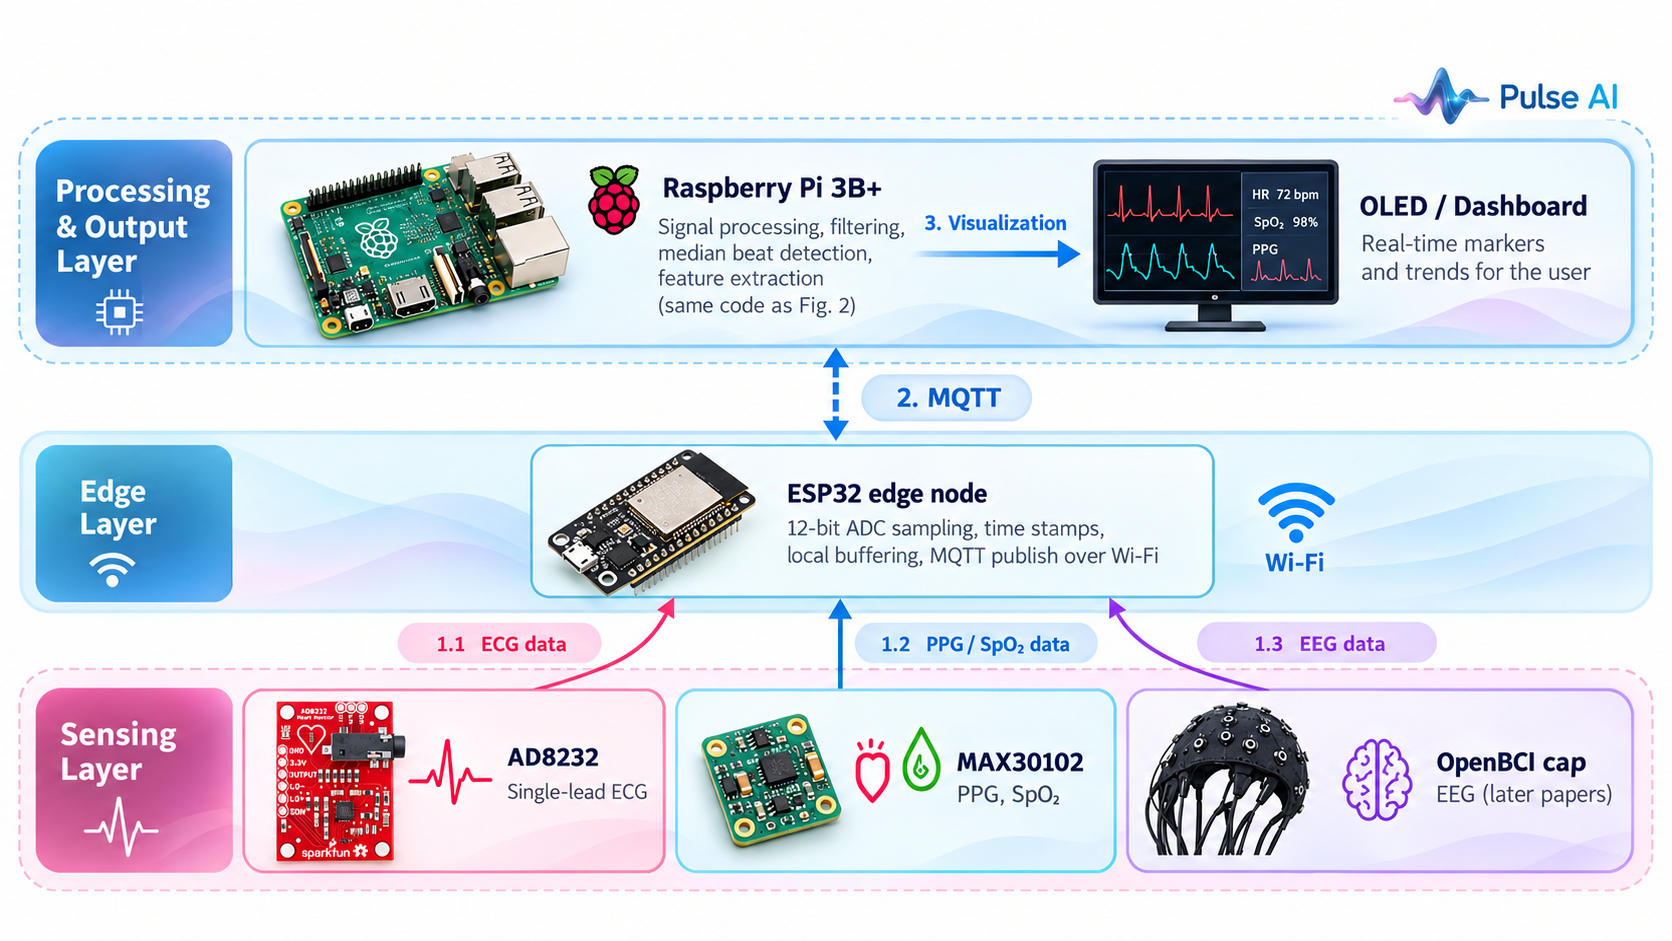
\includegraphics[width=0.85\columnwidth]{fig01_system_v1.png}
\caption{PULSE-AI wearable prototype in three layers. Numbered arrows give the
data path. Illustration only: the dashboard values shown are not measurements,
and no result in this paper uses device data.}
\label{fig:device}
\end{figure}

% ===========================================================================
\section{Conclusion}

PULSE-AI v1 measured named atrial and ventricular ECG markers with stated error.
In \nNAll{} PTB-XL ECGs, P duration with the usual 120\,ms threshold did not
separate expert-labelled LAE from matched controls, while PTFV1 and ventricular
markers did (AUROC \nAucRfA; \nAucRfB{} without P-wave markers). Automated P-wave
analysis should report calibrated continuous values rather than thresholds
taken from single-lead reading.

% ===========================================================================
\section*{Declarations}

\textit{Ethics.} Only public, de-identified databases were used (PTB-XL, LUDB and
QTDB, via PhysioNet~\cite{goldberger2000physionet}). No new data were collected
and ethics approval was not required.
\textit{Data availability.} All data are openly available on PhysioNet; code
is available at the repository given in Section~\ref{sec:software}.
\textit{Funding.} This work was supported by Dawood University of Engineering and Technology and by the authors\textquotesingle{} own funds.
\textit{Use of AI tools.} AI-based tools were used to assist with code development,
language editing and preparation of Figs.~\ref{fig:chain}, \ref{fig:pipeline}, \ref{fig:flow} and~\ref{fig:device}.
The authors checked all content, analyses and references and take full
responsibility for them.
\textit{Competing interests.} The authors declare no competing interests.

\bibliographystyle{IEEEtran}
\bibliography{refs}

\end{document}
